% This template was partially made with assistance from Microsoft Co-pilot

% ------------------------------------------------------------------
% CAPSTONE SOFTWARE REQUIREMENTS SPECIFICATION (SRS)

% 
% This template is inspired by IEEE 29148 but simplified for use in 
% a senior software engineering capstone project. 
% 
% The goal is not to maximize document length. 
% The goal is to produce a clear, testable, and traceable set of 
% requirements that can guide design, implementation, and testing. 
% 
% Recommended workflow: 
% Stakeholder Requirements 
% -> 
% Use Cases 
% -> 
% Functional Requirements 
% -> 
% Acceptance Tests (will be in your VnV plan)
% -> 
% Traceability Matrix (will excluded traceability for tests, that will be in the VnV plan)
% 
% Students should update this document throughout the project. 
% ------------------------------------------------------------------

\documentclass[12pt]{article}

\usepackage{amsmath, mathtools}
\usepackage{amsfonts}
\usepackage{amssymb}
\usepackage{graphicx}
\usepackage{colortbl}
\usepackage{xr}
\usepackage{hyperref}
\usepackage{longtable}
\usepackage{xfrac}
\usepackage{tabularx}
\usepackage{float}
\usepackage{siunitx}
\usepackage{booktabs}
\usepackage{caption}
\usepackage{pdflscape}
\usepackage{afterpage}

\usepackage[round]{natbib}

%\usepackage{refcheck}

\hypersetup{
    bookmarks=true,         % show bookmarks bar?
      colorlinks=true,       % false: boxed links; true: colored links
    linkcolor=red,          % color of internal links (change box color with linkbordercolor)
    citecolor=green,        % color of links to bibliography
    filecolor=magenta,      % color of file links
    urlcolor=cyan           % color of external links
}

\input{../Comments.text}
\input{../Common.text}

% Used so that cross-references have a meaningful prefix

\newcounter{srnum} %Stakeholder Requirement (SR) Number
\newcommand{\srthesrnum}{SR\thesrnum}
\newcommand{\srref}[1]{SR\ref{#1}}

\newcounter{ucnum} %Use Case (UC) Number
\newcommand{\uctheucnum}{UC\theucnum}
\newcommand{\ucref}[1]{UC\ref{#1}}

\newcounter{reqnum} %Functional Requirement (FR) Number
\newcommand{\rthereqnum}{FR\thereqnum}
\newcommand{\rref}[1]{FR\ref{#1}}

\newcounter{nfrnum} %Non-Functional Requirement (NFR) Number
\newcommand{\rthenfrnum}{NFR\thenfrnum}
\newcommand{\nfrref}[1]{NFR\ref{#1}}

\newcounter{lcnum} %Likely Change (LC) Number
\newcommand{\lthelcnum}{LC\thelcnum}
\newcommand{\lcref}[1]{LC\ref{#1}}

\usepackage{fullpage}

\begin{document}

\title{Software Requirements Specification for \progname: subtitle describing software} 
\author{\authname}
\date{\today}
	
\maketitle

~\newpage

\pagenumbering{roman}

\tableofcontents

~\newpage

\section*{Revision History}

\begin{tabularx}{\textwidth}{p{3cm}p{2cm}X}
\toprule {\bf Date} & {\bf Version} & {\bf Notes}\\
\midrule
Date 1 & 1.0 & Notes\\
Date 2 & 1.1 & Notes\\
\bottomrule
\end{tabularx}

~\\
\plt{All capstone SRS documents should have a reflection appendix.}

\newpage

\pagenumbering{arabic}

\plt{This SRS template is based on the IEEE template, with input from co-pilot
  and S. Smith. It will get you started.  You should not modify the section
  headings, without first discussing the change with the course instructor.
  Modification means you are not following the template, which loses some of the
  advantage of a template, especially standardization.}

\plt{Feel free to change the appearance of the report by modifying the LaTeX
  commands.}

\plt{This template document assumes that a single program is being documented.
  If you are documenting a family of models, you should start with a commonality
  analysis.}

\plt{The SRS is not generally written, or read, sequentially.  The SRS is a
  reference document.  It is generally read in an ad hoc order, as the need
  arises.}

\plt{Guiding principles for the SRS document:
\begin{itemize}
\item Do not repeat the same information at the same abstraction level.  If
  information is repeated, the repetition should be at a different abstraction
  level.
\end{itemize}
}

\plt{The template description comments should be disabled before submitting this
  document for grading.}

\plt{You can borrow any wording from the text given in the template.  It is part
  of the template, and not considered an instance of academic integrity.  Of
  course, you need to cite the source of the template.}

\plt{When the documentation is done, it should be possible to trace back to the
  source of every piece of information.  Some information will come from
  external sources, like terminology.}

\plt{An SRS document should have the following qualities: unambiguous,
  consistent, complete, validatable, abstract and traceable.}

\plt{The overall goal of the SRS is that someone can learn,
  understand and verify the captured domain knowledge.  They should not have to
  trust the authors of the SRS on any statements.  They should be able to
  independently verify/derive every statement made.}

% ============================================================== 
\section{Introduction} 
% ==============================================================

\plt{Explain what system is being specified. State purpose, users, and project goals.}

\plt{Introduce the name of your software as \progname{}.  Using \progname{} as
a command lets you change the name if necessary and have the change propagate to
all documents.}

\plt{Include a reference to the template this work is based on.  \citet{ISOIECIEEE29148_2018}
justifies the SRS structure and \citet{ISOIECIEEE15288_2023} provides the
broader life-cycle context that underlines modern requirements engineering
practice.}

\subsection{Purpose}

\plt{State the purpose of the system.}

\plt{The purpose should be in the context of the project itself, not in the
  context of this course. Although the ``purpose'' of the document is to get a
  grade, you should not mention this.  Instead, ``fake it'' as if this is a real
  project.}

\progname{} is intended to solve ... \plt{What problem does your program solve?
The description here should be in the problem space, not the solution space.}

\subsection{Scope}
\plt{Briefly describe:
\begin{itemize}
  \item Problem being solved
  \item Intended users
  \item Major functionality
  \item Expected benefits
  \item Clarifying the scope often means saying what the software doesn't do
\end{itemize}
}

\plt{The scope section is relevant for understanding the boundaries of the system. It is also relevant for later determining typical values of inputs. The scope should make it clear what inputs are reasonable to expect. This is a distinction between scope and context (context is a later section).  Scope affects the inputs while context affects how the software will be used.}

TODO

\subsection{Stakeholders}
\begin{itemize}
\item Customer
\item End Users
\item Project Sponsor
\item Development Team
\item Administrators
\end{itemize}

\subsection{Definitions and Acronyms}

\plt{This section provides the meaning of the different words and phrases used
  in the domain of the problem.}

\begin{longtable}{p{0.25\textwidth} p{0.65\textwidth}}
\toprule
Term & Definition\\
\midrule
TODO & TODO\\
\bottomrule
\caption{Definitions and Acronyms} \label{tab:DefinitionsAndAcronyms}
\end{longtable}

\subsection{Characteristics of Intended Reader} \label{sec_IntendedReader}

\plt{This section summarizes the skills and knowledge of the readers of the
  SRS.  It does NOT have the same purpose as the ``User Characteristics''
  section (Section~\ref{SecUserCharacteristics}).  The intended readers are the
  people that will read, review and maintain the SRS.  They are the people that
  will conceivably design the software that is intended to meet the
  requirements.  The user, on the other hand, is the person that uses the
  software that is built.  They may never read this SRS document.  Of course,
  the same person could be a ``user'' and an ``intended reader.''}

\plt{The intended reader characteristics should be written as unambiguously and
  as specifically as possible.  Rather than say, the user should have an
  understanding of physics, say what kind of physics and at what level.  For
  instance, is high school physics adequate, or should the reader have had a
  graduate course on advanced quantum mechanics?}

% ============================================================== 
\section{System Overview}

This section provides general information about the system.  It identifies the
problem, the vision, and the interfaces between the system and its environment.
This section also describes user characteristics and lists the system
constraints.

\plt{The purpose of this section is to provide general information about the
  system so that the specific requirements in the later sections will be easier to
  understand. The general system description section is designed to be
  changeable independent of changes to the functional requirements documented in
  the specific system description. The general system description provides a
  context for a family of related models.  The general description can stay the
  same, while specific details are changed between family members.}

\subsection{Problem Statement}

\plt{Current situation, problem, impact, desired improvement.  You will likely borrow some text from your problem description document.}

TODO

\subsection{Product Vision}

\plt{A clear and concise statement of the product's purpose and goals.}

\plt{The goal statements are functional and nonfunctional objectives that system
  under consideration should achieve. Goals provide criteria for sufficient
  completeness of a requirements specification and for requirements pertinence.
  Goals will be refined by requirements.  The goals are written abstractly, with
  a minimal amount of technical language.  They should be understandable by
  non-domain experts.}

\plt{You will likely borrow from your goal statements in your problem
description document.}

TODO
  
\subsection{System Context}

\plt{Include users, external systems, APIs, databases, and third-party services.}

\plt{Your system context will include a figure that shows the abstract view of
  the software.  In some cases the diagram will show other external
  entities, besides the user.  For instance, when the software product is a
  library, the user will be another software program, not an actual end user.
  If there are system constraints that the software must work with external
  libraries, these libraries can also be shown on the System Context diagram.
  They should only be named with a specific library name if this is required by
  the system constraint.}

\begin{figure}[h!]
\begin{center}
 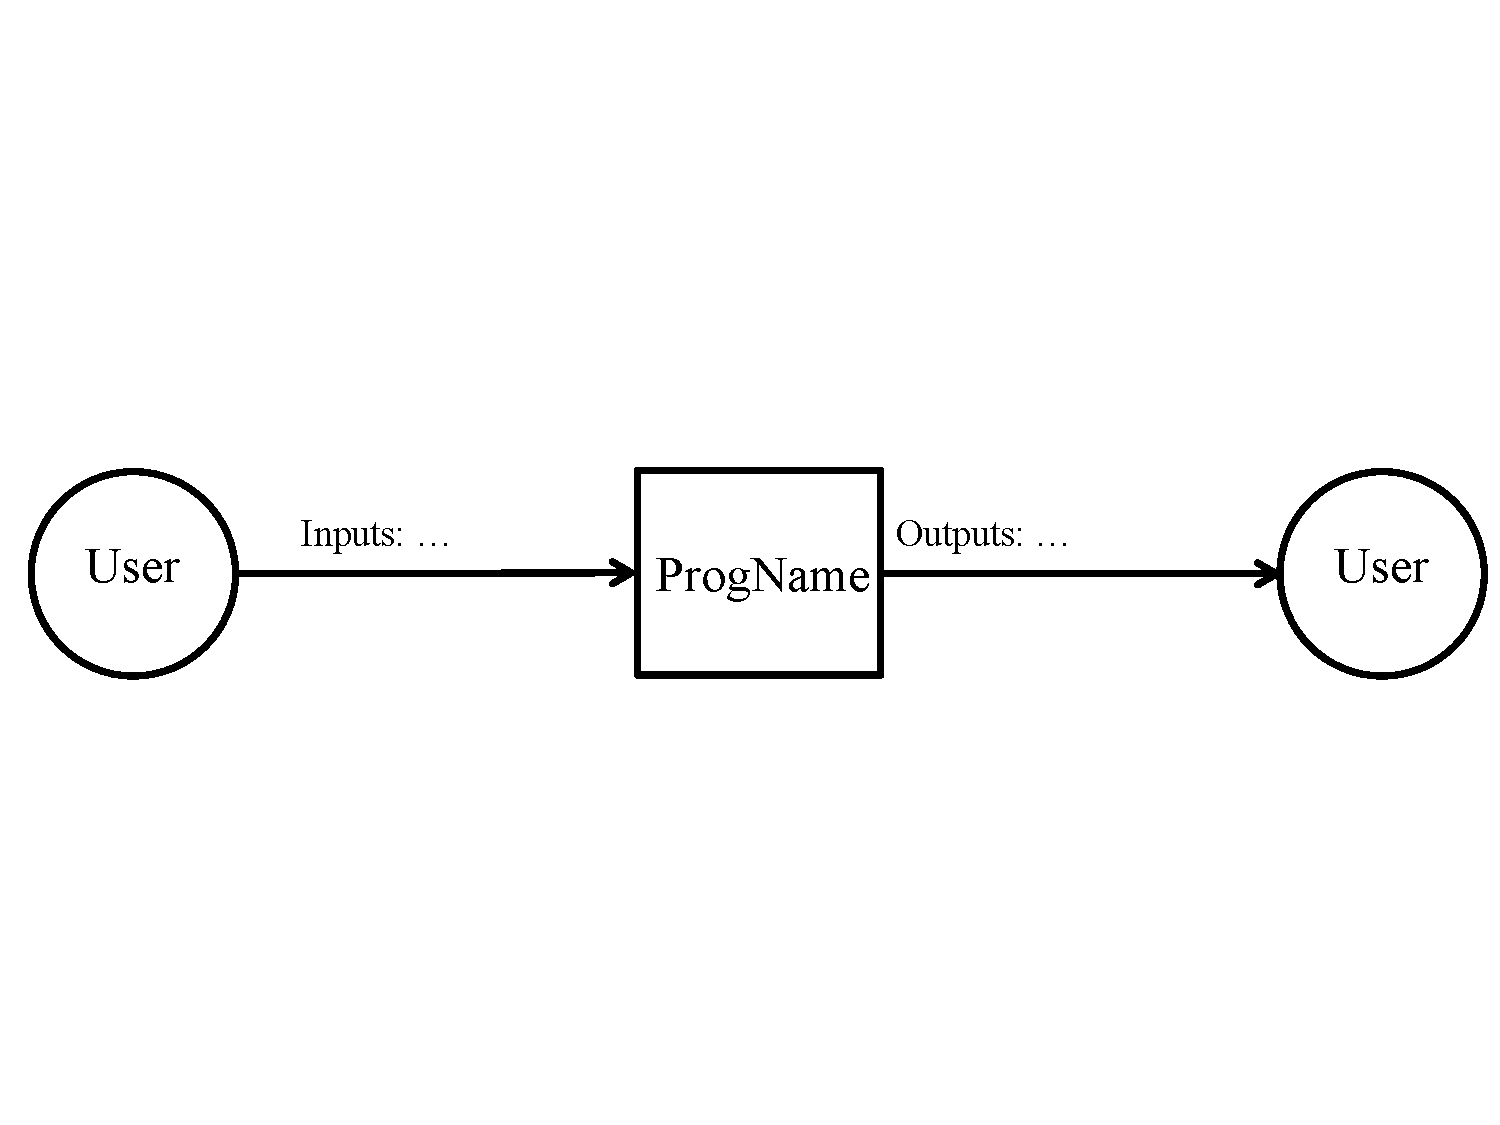
\includegraphics[width=0.6\textwidth]{SystemContextFigure}
\caption{System Context}
\label{Fig_SystemContext} 
\end{center}
\end{figure}

\plt{For each of the entities in the system context diagram its responsibilities
  should be listed.  Whenever possible the system should check for data quality,
  but for some cases the user will need to assume that responsibility.  The list
  of responsibilities should be about the inputs and outputs only, and they
  should be abstract.  Details should not be presented here.  However, the
  information should not be so abstract as to just say ``inputs'' and
  ``outputs''.  A summarizing phrase can be used to characterize the inputs.
  For instance, saying ``material properties'' provides some information, but it
  stays away from the detail of listing every required properties.}

\begin{itemize}
\item User Responsibilities:
\begin{itemize}
\item 
\end{itemize}
\item \progname{} Responsibilities:
\begin{itemize}
\item Detect data type mismatch, such as a string of characters instead of a
  floating point number
\item 
\end{itemize}
\end{itemize}

\plt{Identify in what context the software will typically be used.  Is it for
exploration? education? engineering work? scientific work?. Identify whether it
will be used for mission-critical or safety-critical applications.} 

\plt{This additional context information is needed to determine how much effort
should be devoted to the rationale section.  If the application is
safety-critical, the bar is higher.  This is currently less structured, but
analogous to, the idea to the Automotive Safety Integrity Levels (ASILs) that
McSCert uses in their automotive hazard analyses.}

\subsection{User Characteristics} \label{SecUserCharacteristics}

\plt{This section summarizes the knowledge/skills expected of the user.
  Measuring usability, which is often a required non-function requirement,
  requires knowledge of a typical user.  As mentioned above, the user is a
  different role from the ``intended reader,'' as given in
  Section~\ref{sec_IntendedReader}.  As in Section~\ref{sec_IntendedReader}, the
  user characteristics should be specific an unambiguous.  For instance, ``The
  end user of \progname{} should have an understanding of undergraduate Level 1
  Calculus and Physics.''}

\subsection{System Constraints}

\plt{System constraints differ from other type of requirements because they
  limit the developers' options in the system design and they identify how the
  eventual system must fit into the world. This is the only place in the SRS
  where design decisions can be specified.  That is, the quality requirement for
  abstraction is relaxed here.  However, system constraints should only be
  included if they are truly required.}

\plt{This is where you would mention platform constrains, and licensing
restrictions.}

% ============================================================== 
\section{Stakeholder Requirements}

\plt{Technology-independent requirements.  These come from statements made by
the stakeholders.  You will find these through interviews and surveys.  They are
often expressed in natural language.  They are not necessarily testable, but
they should be verifiable.}

\plt{The stakeholder requirements are numbered so that you can have traceability to other parts of your document.}

\noindent \begin{itemize}

\item[SR\refstepcounter{srnum}\thesrnum \label{SR_Label1}] TODO

\item[SR\refstepcounter{srnum}\thesrnum \label{SR_Label2}] TODO

\item[SR\refstepcounter{srnum}\thesrnum \label{SR_Label3}] TODO

\end{itemize}

\plt{You should give your SRs meaningful labels, so that you can refer to them
in other parts of the SRS.  The label names should be meaningful mnemonics, not
numbers.}

% ============================================================== 
\section{User Personas}
\plt{Create 2-5 realistic personas.
  Personas are fictional characters that represent the different user types that
  might use your software.  They are used to help understand the users'
  needs, experiences, behaviors and goals.  They are not real people, but they
  should be based on real data collected from user research.}

\subsection{Persona 1}
\begin{itemize}
\item Name:
\item Description:
\item Goals:
\item Frustrations:
\item Technical Ability:
\end{itemize}

\subsection{Persona 2}
\begin{itemize}
\item Name:
\item Description:
\item Goals:
\item Frustrations:
\item Technical Ability:
\end{itemize}

% ============================================================== 
\section{Use Cases}
\plt{Use cases are a way to describe the interactions between users and the system.
  They are typically written in natural language and describe the steps that a
  user takes to achieve a specific goal.  Use cases can be used to identify
  functional requirements and to create test cases.}  
\plt{Typically 8-15 substantial use cases.}

\refstepcounter{ucnum} \label{UC_Label1}
\subsection{\ucref{UC_Label1}: Example Use Case}

\textbf{Primary Actor}

TODO

\textbf{Preconditions}
\begin{itemize}
\item TODO
\end{itemize}

\textbf{Main Success Scenario}
\begin{enumerate}
\item TODO
\item TODO
\item TODO
\end{enumerate}

\textbf{Alternative Flows}
\begin{itemize}
\item TODO
\end{itemize}

\textbf{Postconditions}
\begin{itemize}
\item TODO
\end{itemize}

% ============================================================== 
\section{Functional Requirements}
\plt{Functional requirements describe what the system should do.  They are typically
expressed as a set of conditions or capabilities that the system must have.  These
requirements are usually derived from the stakeholder requirements and use cases.}

\plt{Use SHALL statements. Requirements must be atomic, testable, and traceable.}

\noindent \begin{itemize}

\item[FR\refstepcounter{reqnum}\thereqnum \label{FR_Label1}:] The system shall ...

\item[FR\refstepcounter{reqnum}\thereqnum \label{FR_Label2}:] The system shall ...

\item[FR\refstepcounter{reqnum}\thereqnum \label{FR_Label3}:] The system shall ...

\end{itemize}

\plt{The requirements are given labels so that they can be referenced in other
parts of the SRS.  The label names should be meaningful mnemonics, not numbers.}

% ============================================================== 
\section{Data Requirements}

\plt{The Data Requirements section describes what information the system must manage.
  It includes the major data entities, their attributes, and the relationships
  between them.  It also includes a data dictionary that defines the meaning of
  each attribute.}

\subsection{Major Data Entities}

\plt{What information must exist for the system to accomplish its goals?}

\plt{For each entity, provide a short explanation.}

\begin{itemize}
\item User
\item Song
\item Session
\item Report
\end{itemize}

\subsection{Data Dictionary}

\plt{For each entity, define all important attributes.}

\begin{longtable}{p{0.20\textwidth} p{0.20\textwidth} p{0.45\textwidth}}
\toprule
Attribute & Type & Description\\
\midrule
user\_id & UUID & Unique identifier\\
email & String & User email address\\
\bottomrule
\caption{Data Dictionary} \label{tab:DataDictionary}
\end{longtable}

\subsection{Privacy and Data Retention}

\plt{Discuss storage, retention, deletion, privacy controls,
 consent, encryption, and compliance requirements.}

TODO

% ============================================================== 
\section{Non-Functional Requirements}

\plt{You may have to add other NFRs.}

\plt{List your nonfunctional requirements.  You may consider using a fit
  criterion to make them verifiable.}

\plt{The goal is for the nonfunctional requirements to be unambiguous, abstract
  and verifiable.  This isn't easy to show succinctly, so a good strategy may be
to give a ``high level'' view of the requirement, but allow for the details to
be covered in the Verification and Validation document.}

\plt{An absolute requirement on a quality of the system is rarely needed.  For
  instance, an accuracy of 0.0101 \% is likely fine, even if the requirement is
  for 0.01 \% accuracy.  Therefore, the emphasis will often be more on
  describing now well the quality is achieved, through experimentation, and
  possibly theory, rather than meeting some bar that was defined a priori.}

\plt{You do not need an entry for correctness in your NFRs.  The purpose of the
  SRS is to record the requirements that need to be satisfied for correctness.
  Any statement of correctness would just be redundant. Rather than discuss
  correctness, you can characterize how far away from the correct (true)
  solution you are allowed to be.  This is discussed under accuracy.}

\noindent \begin{itemize}

\item[NFR\refstepcounter{nfrnum}\thenfrnum \label{NFR_Accuracy}:]
  \textbf{Accuracy} \plt{Characterize the accuracy by giving the context/use for
    the software.  Maybe something like, ``The accuracy of the computed
    solutions should meet the level needed for $<$engineering or scientific
    application$>$.  The level of accuracy achieved by \progname{} shall be
    described following the procedure given in Section~X of the Verification and
    Validation Plan.''  If you do this provide a link to the VnV plan.}

\item[NFR\refstepcounter{nfrnum}\thenfrnum \label{NFR_Usability}:] \textbf{Usability}
  \plt{Characterize the usability by giving the context/use for the software.
    You should likely reference the user characteristics section.  The level of
    usability achieved by the software shall be described following the
    procedure given in Section~X of the Verification and Validation Plan.  Include a link to the VnV plan.}

\item[NFR\refstepcounter{nfrnum}\thenfrnum \label{NFR_Maintainability}:]
  \textbf{Maintainability} \plt{The effort required to make any of the likely
    changes listed for \progname{} should be less than FRACTION of the original
    development time.  FRACTION is then a symbolic constant that can be defined
    at the end of the report.}

\item[NFR\refstepcounter{nfrnum}\thenfrnum \label{NFR_Portability}:]
  \textbf{Portability} \plt{This NFR is easier to write than the others.  The
    systems that \progname{} should run on should be listed here.  When possible
    the specific versions of the potential operating environments should be
    given.  To make the NFR verifiable a statement could be made that the tests
    from a given section of the VnV plan can be successfully run on all of the
    possible operating environments.}

\item Other NFRs that might be discussed include verifiability,
  understandability, reusability, performance, reliability and availability, security, and accessibility.  You may have to add other NFRs.

\end{itemize}

% ============================================================== 
\section{AI and Machine Learning Requirements}

\plt{Refer to
\href{https://gitlab.cas.mcmaster.ca/courses/capstone/-/blob/main/Lectures/Lxx_DrMosserGuestLecture/2026_09_Capstone.pdf?ref_type=heads}{Dr.
Mosser's guest lecture} on AI requirements.}

\plt{Include only when applicable.}

\subsection{Model Inputs}

TODO

\subsection{Model Outputs}

TODO

\subsection{Evaluation Metrics}

\plt{Accuracy, Precision, Recall, F1, BLEU, WER, etc.}

TODO

\subsection{Known Limitations}

\plt{Explicitly document expected failure modes.}

TODO

% ============================================================== 
\section{Requirements Traceability Matrices}

\plt{The Requirements Traceability Matrix (RTM) is a table that shows the
relationship between different types of requirements. It is used to ensure that
all requirements are traceable and that no requirements are missed. The typical
flow is: Stakeholder Need -> Use Case -> Requirement}

\plt{There is also a traceability matrix between functional and nonfunctional
  requirements. The purpose of some FRs is to satisfy NFRs.  Therefore, it is
  important to show the relationship between the two.}

\plt{Further traceability to test cases and modules will be given in other
documents.}

\begin{longtable}{p{0.15\textwidth} p{0.15\textwidth} p{0.20\textwidth} p{0.20\textwidth}}

\toprule
Stakeholder Req & Use Case & Functional Req \\
\midrule
\srref{SR_Label1} & \ucref{UC_Label1} & \rref{FR_Label1} \\
\bottomrule

\caption{Traceability Between Stakeholder Requirements, Use Cases, and
Functional Requirements} \label{tab:SR2UC2FRtm}
\end{longtable}

\begin{longtable}{p{0.20\textwidth} p{0.20\textwidth}}

\toprule
Functional Req & Nonfunctional Req \\
\midrule
\rref{FR_Label1} & \nfrref{NFR_Accuracy} \\
\bottomrule
\caption{Traceability Between Functional and Nonfunctional Requirements}
\label{tab:FR2Rtm}

\end{longtable}

% ============================================================== 

\section{Rationale}

\plt{Provide a rationale for the decisions made in the documentation.  Rationale
should be provided for scope decisions, functional requirements, nonfunctioanl
requirements, data requirements, and AI requirements.  You don't need a
rationale for everything, ust the major decisions that are not obvious.  You
should have traceability to the entities in the document that you are
referencing.}

\section{Likely Changes}    

\noindent \begin{itemize}

\item[LC\refstepcounter{lcnum}\thelcnum\label{LC_meaningfulLabel}:] \plt{Give
    the likely changes, with traceability to the entity that is likely to change.}

\end{itemize}

\section{Unlikely Changes}    

\noindent \begin{itemize}

\item[LC\refstepcounter{lcnum}\thelcnum\label{LC_meaningfulLabel}:] \plt{Give
    the unlikely changes.  The design can assume that the changes listed will
    not occur.}

\end{itemize}

\newpage{}

\section{Appendices}

\subsection{Appendix A: Additional Materials}

TODO

\subsection{Appendix B: Development Plan}

\plt{This section is optional.  It is used to explain the plan for developing
  the software.  In particular, this section gives a list of the order in which
  the requirements will be implemented.  In the context of a course  this is
  where you can indicate which requirements will be implemented as part of the
  course, and which will be ``faked'' as future work.  This section can be
  organized as a prioritized list of requirements, or it could show the
  requirements that will be implemented for ``phase 1'', ``phase 2'', etc.}

\subsection{Appendix C: Values of Auxiliary Constants}

\plt{Show the values of the symbolic parameters introduced in the report.}

\plt{The definition of the requirements will likely call for SYMBOLIC\_CONSTANTS.
Their values are defined in this section for easy maintenance.}

\plt{The value of FRACTION, for the Maintainability NFR would be given here.}

TODO

\subsection{Appendix D: Generative AI Disclosure}

\plt{Provide full transparency on how generative AI was used in the creation of
  this document.  This includes any text, figures, or tables that were generated
  by AI.  If any skills were created for AI agents to review the documentation,
  those should be disclosed here.}

\subsection{Appendix E: Reflection}

\plt{This isn't part of the SRS, but it is part of the course.}

The information in this section will be used to evaluate the team members on the
graduate attribute of Lifelong Learning.  

\input{../Reflection.text}

\input{../SRS_Reflection.text}

\newpage

\bibliographystyle {plainnat}
\bibliography {../../refs/References}

\newpage


\end{document}